Wie können Computer so viele unterschiedliche Dinge mit nur Nullen und Einser darstellen? Auf dem Bildschirm sehen wir Texte, Bilder, Videos, die wir noch dazu verändern können.

Vorletzte Woche haben wir gesehen, wie Computer ganze Zahlen speichern und manipulieren. Sie stellen die Zahlen in Basis 2 dar und speichern eine feste Anzahl Bits. Letzte Woche haben wir angefangen, uns mit der Darstellung der reellen Zahlen zu beschäftigen, mit den Fliesskommazahlen. Heute machen wir damit weiter.

Die Fliesskommazahlen, wie wir gesehen haben, sind im Grunde genommen nichts anderes, als die Exponentialschreibweise, die wir schon aus Chemie und Physik kennen: Die signifikanten Stellen werden mit der Basis hoch einen Exponenten multipliziert. Im Unterschied zu Menschen, arbeitet der Computer meistens in der Basis \(2\) statt \(10\) und schränkt die Anzahl der möglichen signifikanten Stellen und Exponenten ein.

Um diese Einschränkungen sichtbar und anfassbar zu machen, hatten wir das ''Kasten-Seil''-Modell eingeführt.

Stellen wir uns reelle Zahlen in Basis 2 vor:

\begin{figure}[H]
\centering
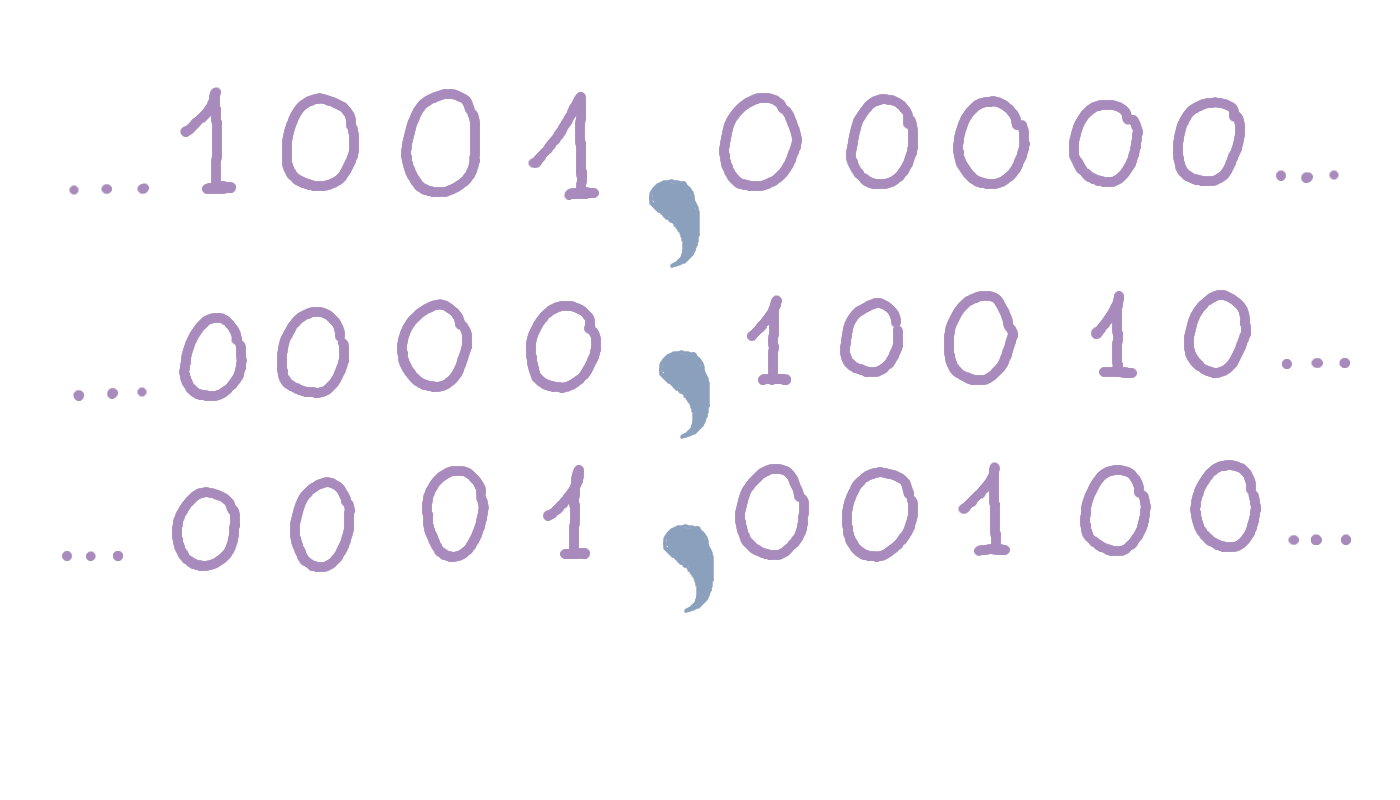
\includegraphics[width=0.65\linewidth]{Pictures/Zahlengerade.png} 
\end{figure}

Die Signifikanten Stellen, die wir speichern wollen, tun wir in einen Kasten.
\begin{figure}[H]
\centering
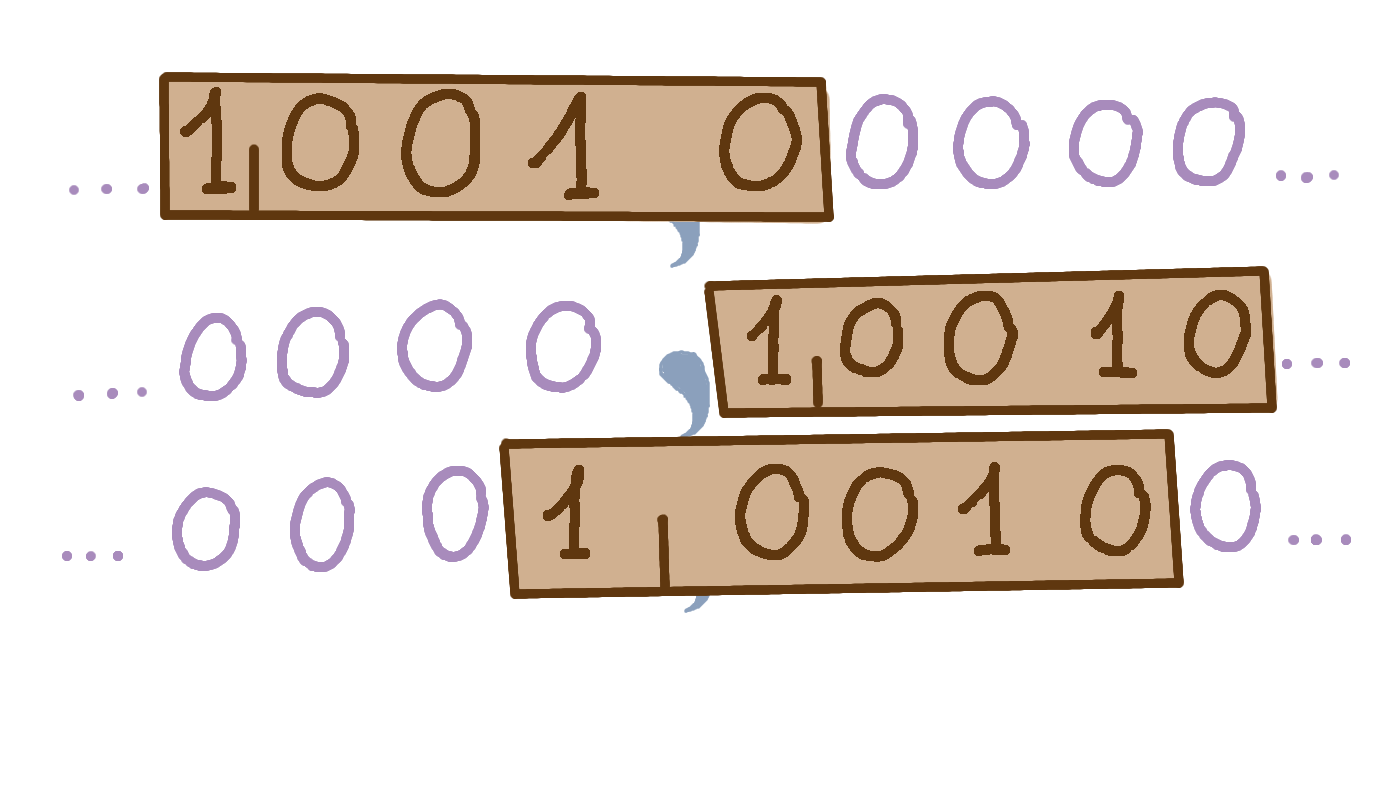
\includegraphics[width=0.65\linewidth]{Pictures/Kasten.png} 
\end{figure}

Um zu wissen, woher wir diese signifikanten Stellen rausgenommen haben, markieren wir auf einem Seil den Abstand bis zum Komma.
\begin{figure}[H]
\centering
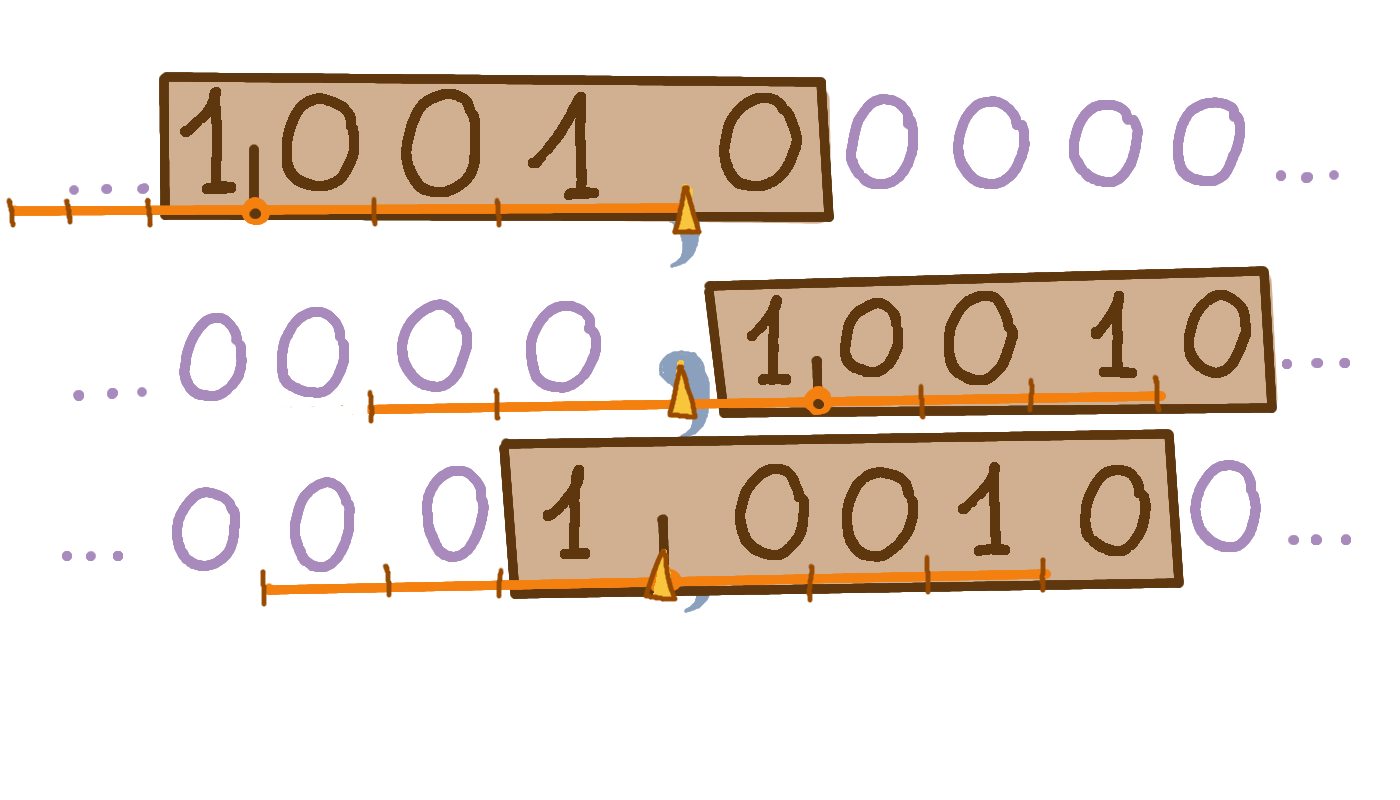
\includegraphics[width=0.65\linewidth]{Pictures/KastenMitSeil.png} 
\end{figure}
Jetzt haben wir alle Informationen gespeichert, die wir brauchen, um diese Zahl wiederherzustellen. Damit diese Darstellung eindeutig ist, verlangen wir, dass das erste Bit der Mantisse eine Eins ist.

Folgende Elemente charakterisieren ein Fliesskommazahlensystem: Die Grösse vom Kasten, d.h. die Mantissenlänge, und die Länge vom Seil, d.h. der Exponentenbereich. Die Bits im Kasten und die Markierung am Seil stellen eine Zahl dar.
\begin{figure}[H]
\centering
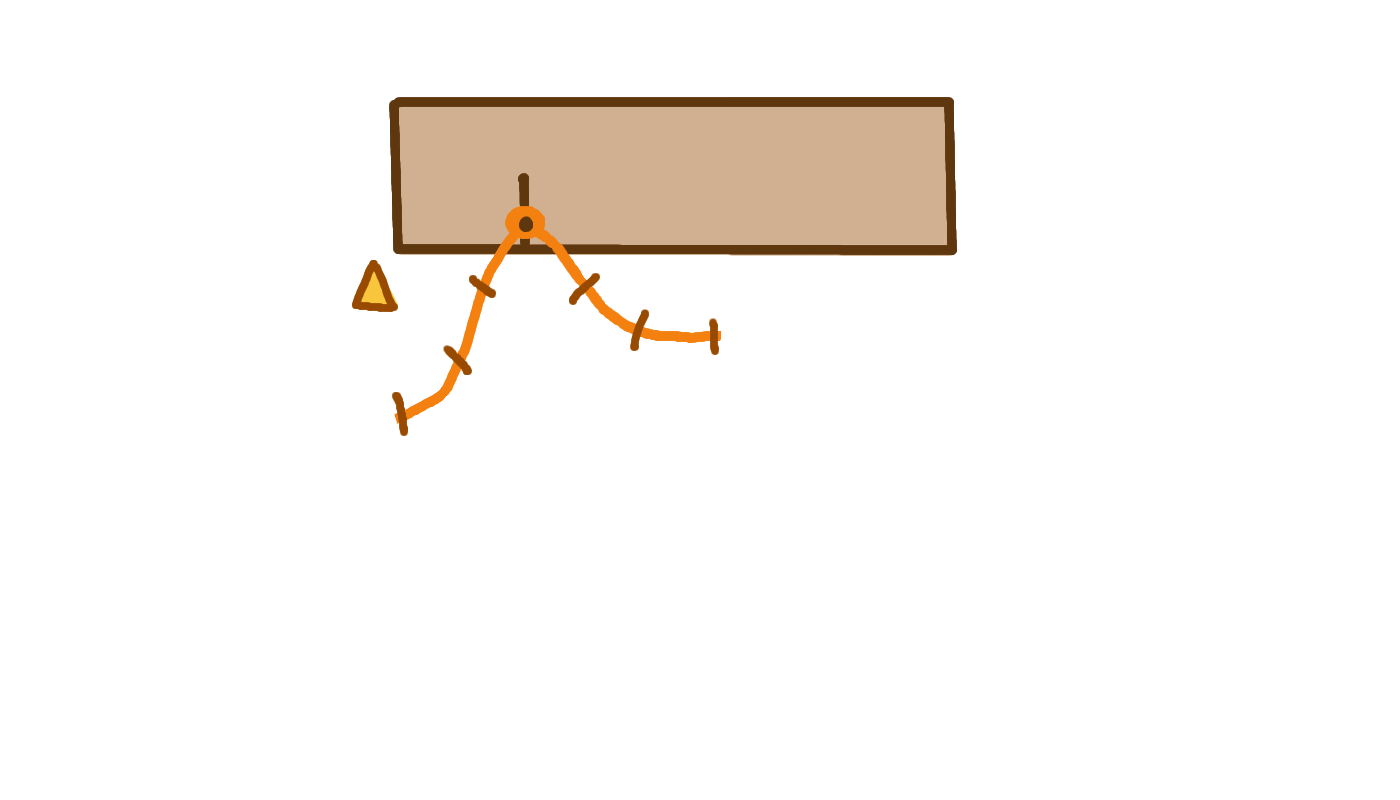
\includegraphics[width=0.75\linewidth]{Pictures/KastenOhneZahlen.png} 
\end{figure}

Der Computer hat intern keine Kasten und keine Seile. Er arbeitet mit Bitmuster. Die Bits werden in \(3\) Bereichen aufgeteilt: Vorzeichen (grün auf dem Bild), Exponent (Orange auf dem Bild) und Mantisse (braun auf dem Bild). Im Mantissenteil werden die Bits aus dem Kasten gespeichert. Im Exponententeil wird die Markierung am Seil kodiert. Im Vorzeichenteil wird das Vorzeichen kodiert (\texttt{0} für positive Zahlen und \texttt{1} für negative).
\begin{figure}[H]
\centering
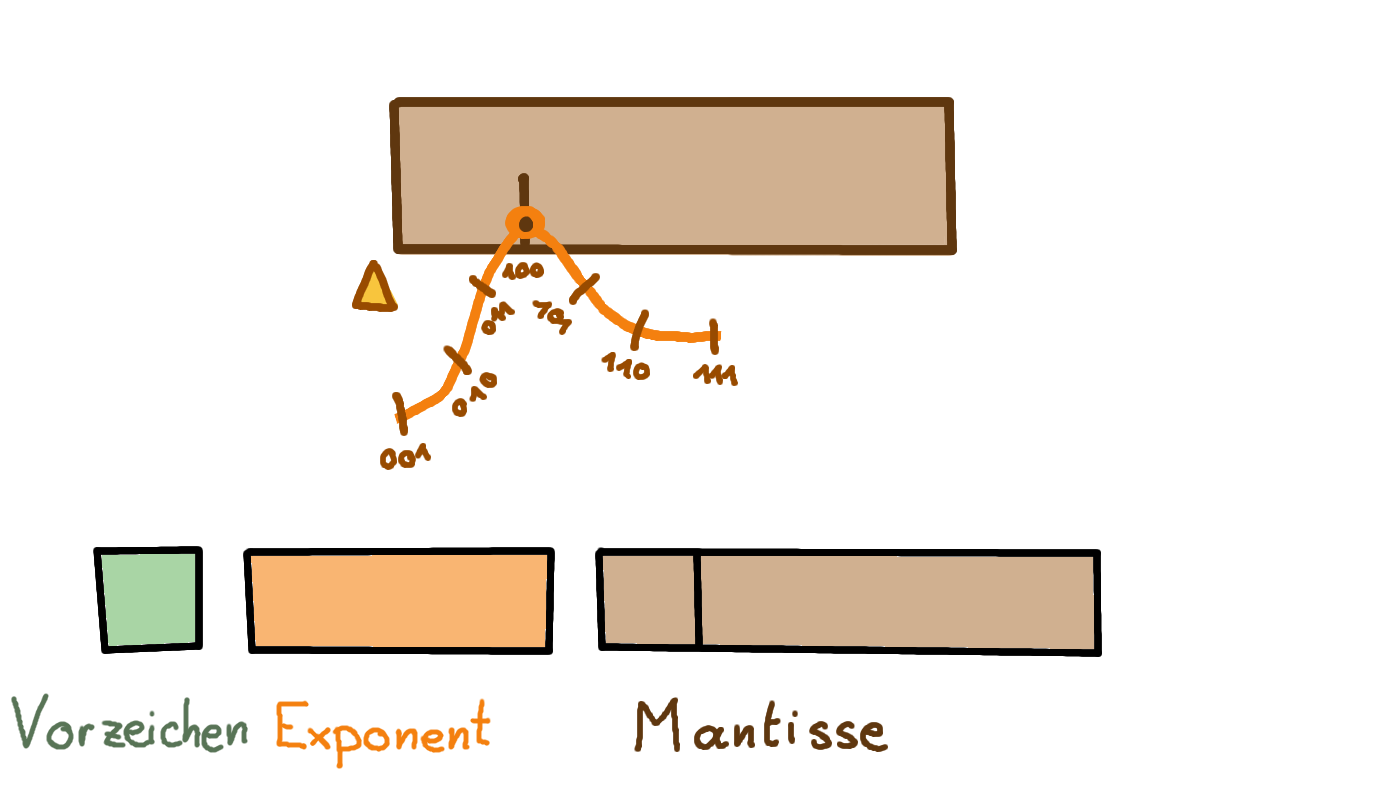
\includegraphics[width=0.75\linewidth]{Pictures/KastenMitSpeicher.png} 
\end{figure}

\begin{beispiel}
Wir werden jetzt zusammen die Zahl \(6.5\) im Fliesskommazahlensystem mit Mantissenlänge \(5\) und Exponenten von \(-3\) bis \(3\) darstellen.

Die reelle Zahl in Basis 2 ist \(110.1\).

Der Kasten hat 5 Plätze. Alle signifikanten Stellen haben dort Platz. Dann verbinden wir das Seil mit dem Komma und setzen eine Markierung. Das lässt sich direkt ins Bitmuster übersetzen: Das Vorzeichen ist positiv, die Kodierung vom Exponenten lässt sich am Seil ablesen, die Mantisse speichert man direkt.
\begin{figure}[H]
\centering
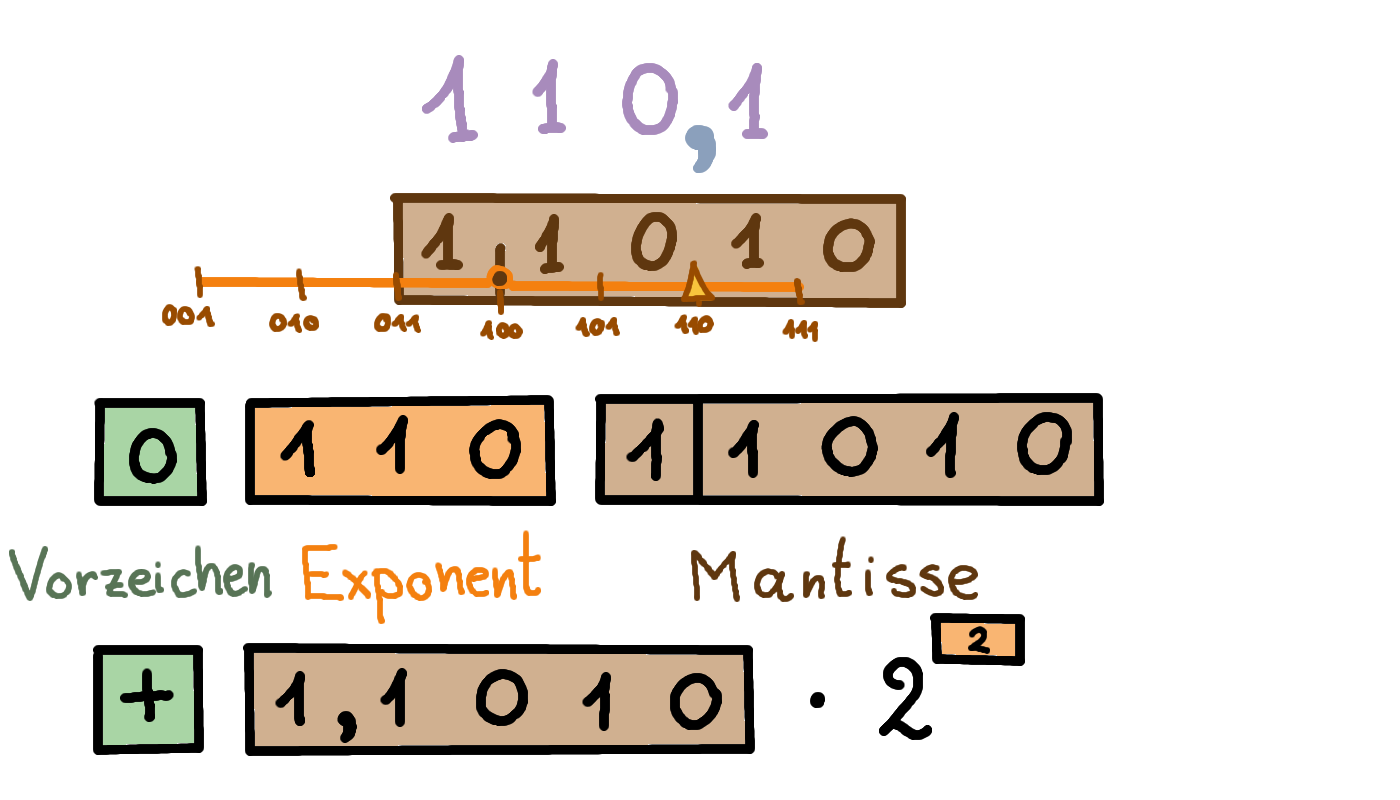
\includegraphics[width=0.75\linewidth]{Pictures/ZahlenDarstellen6-5.png} 
\end{figure}

\end{beispiel}

\begin{beispiel}
Nicht alle Zahlen lassen sich im Fliesskommazahlensystem genau darstellen. Manche müssen gerundet werden.
Zum Beispiel, die Zahl \(10.75\) sieht in Binär so aus: \(1010.11\). Sie hat \(6\) signifikante Stellen, aber nur \(5\) haben in der Mantisse Platz. Die letzte Eins kann nicht gespeichert werden und geht verloren.
\begin{figure}[H]
\centering
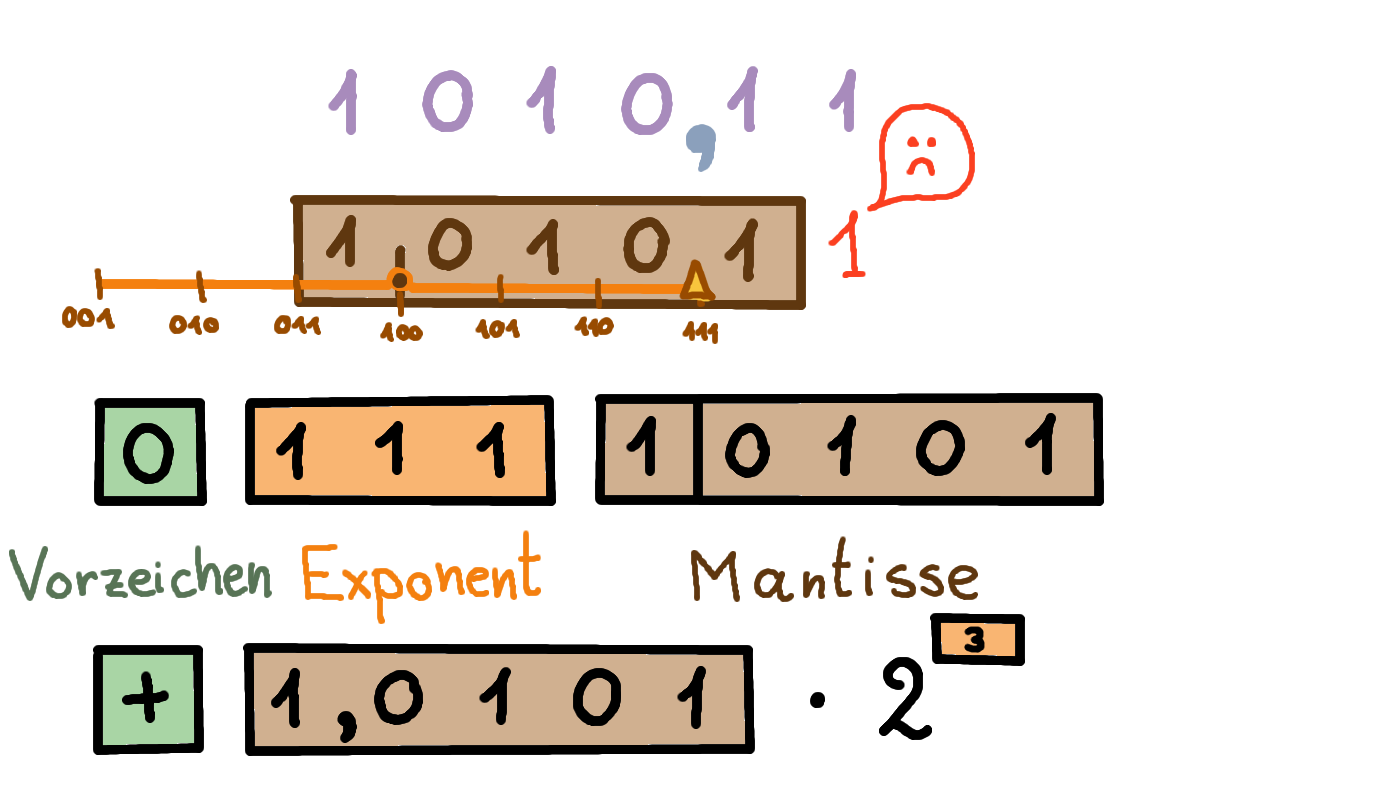
\includegraphics[width=0.75\linewidth]{Pictures/ZahlenDarstellen10-75.png} 
\end{figure}

\end{beispiel}